\documentclass[a4paper,11pt]{article}

\usepackage[english]{babel}
\usepackage{mathrsfs, amssymb, amsmath, amsthm, enumerate}
\usepackage{verbatim,graphicx,geometry,bbm}
%\usetikzlibrary{arrows}
\usepackage[utf8]{inputenc}
\usepackage{authblk}
\usepackage[round]{natbib}
\bibliographystyle{plainnat}

\usepackage{hyperref}

\makeatletter
\def\@biblabel#1{\hspace*{-\labelsep}}
\makeatother
\geometry{left=1in,right=1
in,top=1in,bottom=1in}
\newdimen\dummy
\dummy=\oddsidemargin
\addtolength{\dummy}{72pt}
\marginparwidth=.5\dummy
\marginparsep=.1\dummy


\newcommand{\E}{\mathbb{E}}
\newcommand{\Var}{\mathrm{Var}}
\newcommand{\plim}{\overset{p}{\longrightarrow}}
\newcommand{\dlim}{\overset{d}{\longrightarrow}}

\begin{document}

\section{Parameters}

\subsection{Recap}

\begin{itemize}
\item New ideas are distributed according to a truncated logistic distribution. The location parameter (that equals the mode) is the inventor's position in the technology line and the scale parameter (that determines the variance) is $\tau$.

\item In the theoretical model, the distribution of the cost parameters, $\alpha$, does not influence in the results. In this simulation, I have assumed that $\alpha$ is distributed according to a Weibull distribution with scale parameter $\lambda$ and shape parameter $\kappa$.

The reason I chose this distribution is that it is confined to positive values and is ``flexible" -- depending on parameter values, the Weibull can look like an exponential or a normal distribution.
\end{itemize}

\subsection{Parameter values}

There are 12 parameters in the model, described in table 1. For 6 of those parameters we have attributed values from matching moments in the model to moments in the data\footnote{Those values com from simulating the model with the older version of the code (with a typo).}. Those parameters are described in table 2. For the rest of the model parameters, their values are either normalized or guessed, as described in table 3.

Even though these are not parameters in the model, the initial quality of product lines is also relevant. They are all normalized to 1.

\begin{table}[h!]
\caption{Model Parameters}
\centering
\begin{tabular}{ll}
\hline \hline
Parameter & Interpretation \\ \hline
$\eta^H$ & New technology quality increase. \\
$\eta^M$ & New combination quality increase. \\
$\eta^L$ & Reuse/refinement quality increase. \\
$\tau$ & Scale parameter of the new ideas distribution. \\
$\lambda$ & Scale parameter of the distribution of costs. \\
$\kappa$ & Shape parameter of the distribution of costs. \\
$\xi$ & Determines the fraction of viable combinations in a pool, $1/\xi$.\\
$\gamma$ & Determines the scale of the final goods production function. \\
$\epsilon$ & Determines the elasticity of intertemporal substitution of consumption.\\
$\beta$ & Intertemporal discount factor. \\
$I$ & Number of inventors.\\
$J$ & Number of firms.\\
\hline \hline
\end{tabular}
\end{table}

\begin{table}[h!]
\caption{Parameters taken from moment matching.}
\centering
\begin{tabular}{llll}
\hline \hline
Parameter & Value & Objective function value & Interpretation \\ \hline
$\eta^H$ & 0.15 & 0.026 & New technology benefit \\
$\eta^M$ & 0.03 & 0.026 & New combination benefit \\
$\tau$ & 300 & 0.026 & Shape parameter for idea distribution \\
$\xi$ & 10 & 0.026 & $1/\xi$ is the fraction of viable combinations \\
$\lambda $ & 2.2 & 0.026 & scale parameter of the cost distribution \\
$\kappa $ & 5 & 0.026 & shape parameter of the cost distribution \\
\hline \hline
\end{tabular}
\end{table}

\begin{table}[h!]
\caption{Parameters with normalized or guessed values.}
\centering
\begin{tabular}{lll}
\hline \hline
variable & value & Normalized or guessed \\ \hline
$\eta^L$ & 0 & Normalized. \\
$\gamma$ & 0.7 & Guess (I have no good reason for this number; results are sensitive). \\
$\epsilon$ & 1/2 & Guess (I tried other values as well -- welfare results are sensitive). \\
$\beta$ & 0.954 & $=\frac{1}{1+r}$, with $r = 5\%$. \\
$I$ & 500 & Guess. \\
$J$ & 660 & Sort of guess -- given the other values, this makes the average growth $\approx 2\%$. \\
\hline \hline
\end{tabular}
\end{table}


\section{Counterfactual exercises}

The counterfactual exercise presented here provides a targeted subsidy for \textit{new technology} patents. In the numerical simulation, this subsidy was equivalent to 25\% of the inventor's costs for implementing a new technology. I also assumed that this subsidy is funded with a lump-sum tax on consumption of the final good. In this case, the aggregate final goods market clearing condition is:

\[ Y_t = C_t + \mbox{inventor's costs}_t + \mbox{intermediaty producer's costs}_t + \mbox{subsidy policy's costs}_t \]

\subsection{Numerical results}

The first set of results concerns the changes in aggregate variables, namely GDP, consumption and the numerous costs. The evolution of these variables over time is described in figure 1. Note that the subsidy policy increases all costs, as inventors are producing more patents and increasing the average quality of products, but also increases GDP. Consumption drops at the beginning but quickly recovers and surpasses the ``no subsidy consumption" around the 1900's. Another interesting result is that the policy costs are non-monotonic: they are very high at the beginning, when most patents are defined as new technologies, steadily decrease as the fraction of new technologies decreases, and then increase again around 1950, when the average quality of product lines takes off (see from figure 2 that the fraction of new technologies do not increase at this same period).

Figure 2 displays the changes in patent shares and GDP growth rate when the subsidy policy is introduced. Note that, despite the subsidy policy being targeted towards new technologies, the share of new technologies does not increase too much (probably because having the idea for a new technology is a rare event to begin with). However, the share of new combinations increases substantially! This is the effect of new technologies being born ``hot" -- as more technology lines are born hot, the chances of doing new combinations increase considerably due to the combinatorial aspect of these patents. In response to that, the share of reuses drops considerably as well.

Finally, table 4 has some summary statistics. Note that welfare has increased by a little over 1\%\footnote{This result depends a lot on $\epsilon$ and $\gamma$, and could be negative (e.g. $\epsilon = 2$ makes the welfare gain negative).}, the number of existing technologies more than doubles and average GDP growth increases by around 10\%. The average GDP growth increase is probably mostly due to the initial spike, so the number reported in table 4 is probably overestimating the actual growth.

\begin{table}[h!]
\centering
\caption{Summary statistics of the economy with and without the subsidy policy.}
\input{code/counterfactual_table1.tex}
\end{table}

\begin{figure}[h!]
\centering
\caption{Changes in aggregate variables when a subsidy is implemented.}
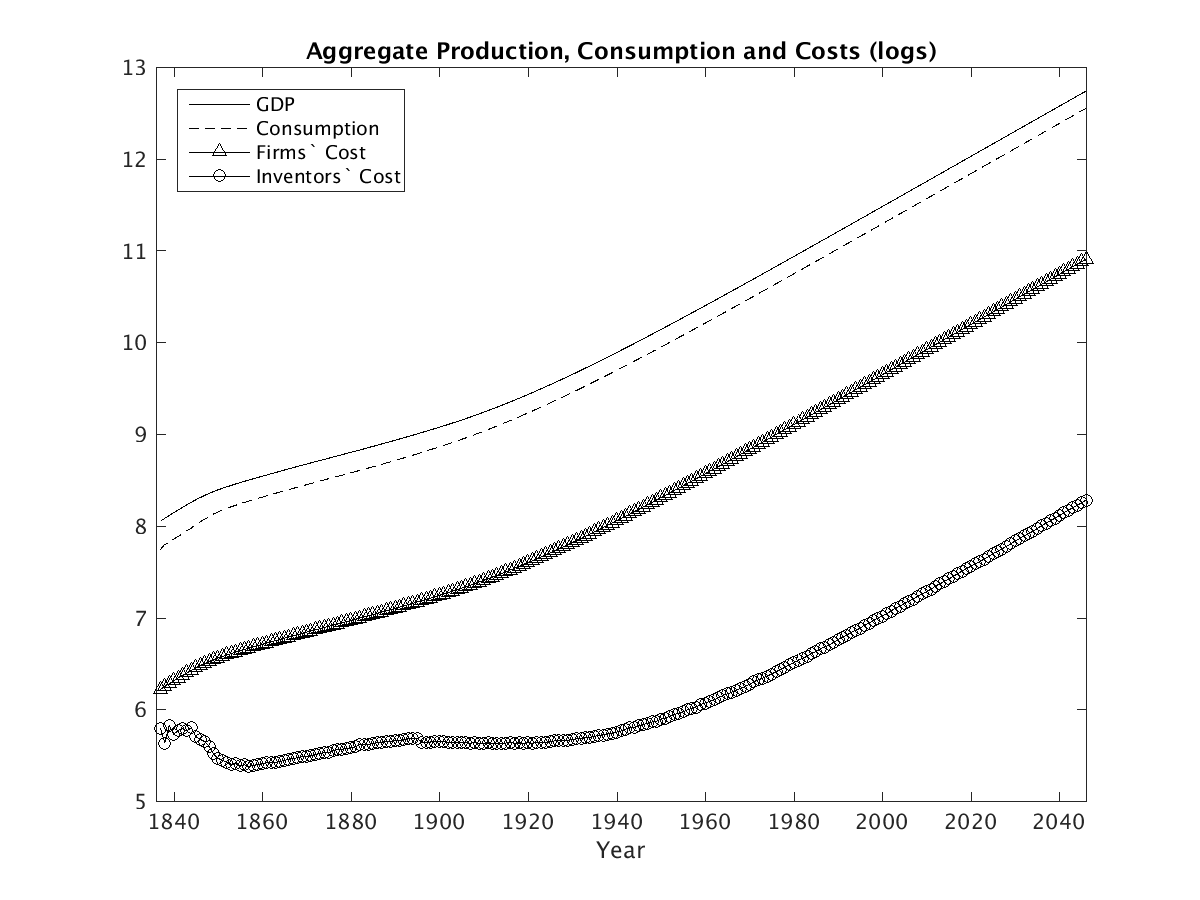
\includegraphics[scale=.8]{code/aggregates}
\end{figure}

\begin{figure}[h!]
\centering
\caption{Changes in patent type fractions when a subsidy is implemented.}
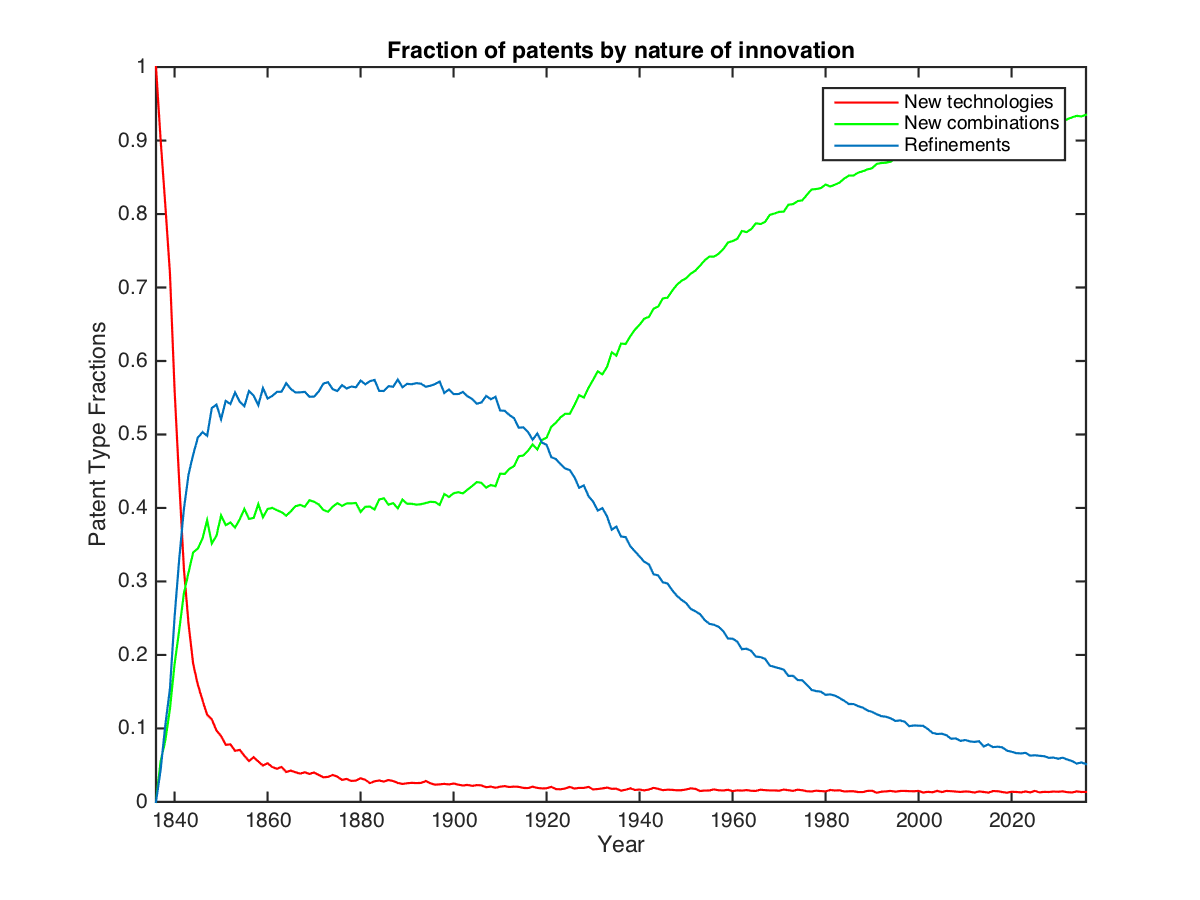
\includegraphics[scale=.8]{code/patents}
\end{figure}

\clearpage

\appendix

\section{Derivations}

\subsection{Growth rate}


There is a final good, produced with technology

\[ Y_t = \frac{L_t^{\gamma}}{1-\gamma}\sum_{j \in \mathcal{J}} q_{jt}^{\gamma}k_{jt}^{1-\gamma}. \]

Labor is inelastic, so $L_t \equiv 1$ and the profit maximization of firms implies $q_{jt} = k_{jt}$. This, in turn, gives

\[ Y_t = \frac{1}{1-\gamma}\sum_{j \in \mathcal{J}}q_{jt}. \]

Finally, we also have that the quality fo the product of a firm evolves according to

\[ q_{j,t+1} = q_{jt} + s_j\bar{q}_t \]
where $s_j$ is the quality of the patent that was purchased and $\bar{q}_t$ is the average quality in year $t$. 

Define the growth rate $g_t$ as

\[ g_t = \frac{Y_{t+1} - Y_t}{Y_t} = \frac{\frac{1}{1-\gamma}\sum_{j \in \mathcal{J}}q_{j,t+1} - \frac{1}{1-\gamma}\sum_{j \in \mathcal{J}}q_{jt}}{\frac{1}{1-\gamma}\sum_{j \in \mathcal{J}}q_{jt}} \]

Plugging in $q_{j, t+1}$, we have
\[ g_t = \frac{\sum_{j \in \mathcal{J}}s_j \bar{q}_t}{\sum_{j \in \mathcal{J}}q_{jt}} \]
and finally, using the definition of $\bar{q}_t$, we get

\[ g_t = \frac{\frac{1}{\mathcal{J}}\sum_{j \in \mathcal{J}}q_{jt}\sum_{j \in \mathcal{J}}s_j}{\sum_{j \in \mathcal{J}}q_{jt}} \]

\[ g_t = \frac{1}{\mathcal{J}}\sum_{j \in \mathcal{J}}s_j \]


\subsection{Consumption and welfare}

From the discussion in section 2, we can write the final goods consumption as

\[ C_t = Y_t - \mbox{inventor's costs}_t - \mbox{intermediaty producer's costs}_t - \mbox{subsidy policy's costs}_t .\]
We know that
\[ Y_t = \frac{1}{1-\gamma}\sum_{j \in \mathcal{J}}q_{jt} \] and that the sum of all intermediary producers' costs is equal to 
\[ (1-\gamma)\sum_{j \in \mathcal{J}}q_{jt}. \]
The cost for an inventor $i$ is
\[ \alpha_i \bar{q}_t ,\]
so that the cost of all inventors is
\[ \sum_{i = 1}^{I}\alpha_i \bar{q}_t.\] In the numerical simulation, this was approximated by
\[ \sum_{k = 1}^{M_t} \mu_k \alpha_{i(k)} \bar{q}_t, \] where $\mu_k$ is the measure of inventors with expertise in product line $k$ and $\alpha_{i(k)}$ is the cost of those inventors (assumed to be constant over product lines).

Finally, the subsidy policy costs are computed as
\[ \sum_{p = 1}^2 \sum_{k = 1}^{M_t} \mathbbm{1}\{\mbox{patent type} = p\}\times \mbox{subsidy}(p) \times \mu_k \times \alpha_{i(k)}  \times \bar{q}_t\]
(recall that the cost of reuse is normalized to zero).

Having all of those quantities, we can compute consumption using the equation at the beginning of this subsection. Welfare is then computed as

\[ W = \sum_{t=1}^T \beta^t \frac{C_t^{1-\epsilon}}{1-\epsilon}. \]









\end{document}